% !TeX program = xelatex
% !TeX TXS-program:xelatex = -shell-escape

\documentclass{article}
\usepackage{xeCJK}
\usepackage[a4paper, left=1cm, right=1cm, top=1cm, bottom=1.5cm]{geometry}    %设置页面边距
\usepackage{graphicx}   %插入图片

\usepackage{minted}     %允许插入代码段。需要在settings.json中"latex-workshop.latex.tools"节点的子节点"name":"xelatex"下面添加"-shell-escape",
% \usepackage{minted} % 引用minted包
\usepackage{caption} % 引用caption包
\usepackage{fvextra} % 引用fvextra包
\DeclareCaptionType{code}[Code Listing][List of Code Listings] % 设置code环境为新的代码环境


%\setCJKmainfont{STHeiti} % 设置字体
%\setCJKsansfont{STHeiti}
%\setCJKmonofont{STHeiti}

\usepackage{amsmath} % 数学公式包
\usepackage{amssymb} % 实数集的包
\usepackage{parskip} % 段落包
\usepackage{setspace} % 行距包
% \setlength{\parindent}{0pt} % 取消段落缩进
\usepackage{titlesec} % 章节标题格式包
\titleformat*{\section}{\large\bfseries} % 设定section标题格式为加粗大号字体
\usepackage{tocloft} % 目录格式包
\renewcommand\cftsecfont{\normalfont\bfseries} % 设定section标题格式为加粗字体
\renewcommand\cftsecpagefont{\normalfont\bfseries} % 目录页码字体
\usepackage{ragged2e} % 左对齐包
\usepackage{hyperref} % 超链接包
\usepackage{array} % 引入 array、表格 包
\hypersetup{colorlinks=true, linkcolor=blue, filecolor=magenta, urlcolor=blue} % 超链接格式设置


\title{常见数学公式}
\author{Lindeci}
\date{\today}

\begin{document}
\maketitle
\tableofcontents

\definecolor{codebgcolor}{HTML}{F8F8F8} % 设置背景颜色

\section{高中数学}
\subsection{三角函数}
$sin(a+b) = \sin a \cos b + \cos a \sin b$ \\
$cos(a+b) = \cos a \cos b - \sin a \sin b$ \\
\subsection{向量}
向量$A(x_1,y_1),B(x_2,y_2),
\begin{bmatrix}
x_1 & x_2 \\
y_1 & y_2
\end{bmatrix}
$ \\
$A \bot B \Leftrightarrow A \cdot B = x_1 x_2   + y_1 y_2 = 0$ \\
$ \cos \theta = \frac {A \cdot B} {\vert A \vert \vert B \vert} =\frac {(x_1 x_2 + y_1 y_2)} {\sqrt{x_1^2+y_1^2} \sqrt{x_2^2+y_2^2}}$ \\
$
A \times B = x_1  y_2 - x_2 y_1 = \mathbf{S}_{abcd} = 
\begin{vmatrix} x_1 & x_2 \\
y_1 & y_2 
\end{vmatrix}
$

\subsection{求导法则}
1、可加性:$(u+v)'=u'+v'$   \\
2、常数因子:$(cu)'=cu'$    \\
3、乘法法则:$(uv)'=u'v+uv'$    \\
4、商法法则:$\left(\frac{u}{v}\right)'=\frac{u'v-uv'}{v^2}$    \\
5、复合函数法则:$(f(g(x)))'=f'(g(x))\cdot g'(x)$   \\

\subsection{导数表}
\begin{table}[htbp]
%    \begin{flushleft} %将表格左对齐
    \centering
    \renewcommand{\arraystretch}{1.8} % 设置表格行高
    \begin{tabular}{|c|c|}
        \hline
        函数 & 导数公式\\
        \hline
        $c$ & $0$\\
        \hline
        $x$ & $1$\\
        \hline
        $x^n$ & $nx^{n-1}$\\
        \hline
        $\sqrt x$ & $\frac{1}{2\sqrt{x}}$\\
        \hline
        $\frac{1}{x}$ & $-\frac{1}{x^2}$\\
        \hline
        $\log_a x$ & $\frac{1}{x\ln a}$\\
        \hline
        $\ln x$ & $\frac{1}{x}$\\
        \hline
    \end{tabular}   %结束表格
    \caption{高中数学的导数表}
%   \end{flushleft} %结束左对齐命令
\end{table}

\subsection{不定积分}
若连续函数 $F(x)$ 在区间 $[a,b]$ 内具有导数 $f(x)$,则记
$$ \int f(x) dx = F(x) + C $$
其中 $C$ 为任意常数。

\subsection{简易积分表}
$ \int x^n \ dx = \frac{1}{n+1} x^{n+1} + C $   \\
$ \int \frac{1}{x} \ dx = \ln |x| + C $   \\
$ \int e^x \ dx = e^x + C $   \\
$ \int a^x \ dx = \frac{a^x}{\ln a} + C $   \\
$ \int \sin x \ dx = -\cos x + C $   \\
$ \int \cos x \ dx = \sin x + C $   \\
$ \int \tan x \ dx = \ln |\sec x| + C $   \\
$ \int \cot x \ dx = \ln |\sin x| + C $   \\
$ \int \sec x \ dx = \ln |\sec x + \tan x| + C $   \\
$ \int \csc x \ dx = \ln |\csc x - \cot x| + C $   \\

\subsection{积分法则}
1. 常数法则 $\quad\int k f(x) dx = k \int f(x) dx + C$   \\
2. 换元法则 $\quad\int f(g(x)) g'(x) dx = \int f(u) du \quad (u=g(x))$   \\
3. 分部积分法则 $\quad\int u v' dx = u v - \int u' v dx$   \\
4. 简单的不定积分 $\quad\int x^n dx = \frac{x^{n+1}}{n+1} + C \quad (n \neq -1)$   \\
5. 指数函数 $\quad\int e^x dx = e^x + C$   \\
6. 正弦函数 $\quad\int \sin x dx = -\cos x + C$   \\
7. 余弦函数 $\quad\int \cos x dx = \sin x + C$   \\
8. 倒数函数 $\quad\int \frac{1}{x} dx = \ln|x| + C$   \\


\subsection{定积分}
定积分是将一个区间上的函数在该区间上的取值乘以区间长度(也就是自变量的取值范围),然后将这些乘积全部加起来,最后形成的一个数。数学符号表达式如下:

$$ \int_a^b f(x)dx $$

其中,aa和bb是定义定积分的区间,f(x)f(x)是在该区间中的函数。

\subsection{定积分的计算公式}
定积分的计算公式是牛顿-莱布尼茨公式,即:
$$ \int_a^b f(x)dx=F(b)-F(a) $$

%--------------------------------------------------------------------------------------------------

\section{线性代数}
\subsection{标量、向量、矩阵和张量} 
广播:$\mathbf{C}=\mathbf{A}+\boldsymbol{b}$,其中C和A是矩阵,b是向量,且$\mathbf{C}_{i,j}=\mathbf{A}_{i,j}+\boldsymbol{b}_j$

例子
\[
\begin{bmatrix}
2 & 3 & 4 \\
5 & 6 & 7 \\
8 & 9 & 10
\end{bmatrix}
+
\begin{bmatrix}
1 \\
2 \\
3
\end{bmatrix}
=
\begin{bmatrix}
2+1 & 3+1 & 4+1 \\
5+2 & 6+2 & 7+2 \\
8+3 & 9+3 & 10+3
\end{bmatrix}
=
\begin{bmatrix}
3 & 4 & 5 \\
7 & 8 & 8 \\
11 & 12 & 13
\end{bmatrix}
\]

--------------------------------------------------------------------------------------------------

\subsection{矩阵和向量相乘}
矩阵乘积
\begin{equation}
    \boldsymbol{C}=\boldsymbol{A}\boldsymbol{B}
\end{equation}
具体地
\begin{equation}
    \mathbf{C}_{i,j}=\sum_{k}\mathbf{A}_{i,k}\mathbf{B}_{k,j}
\end{equation}

\[
\begin{bmatrix}
1 & 2 \\
3 & 4 \\
5 & 6
\end{bmatrix}
\times
\begin{bmatrix}
7 & 8 \\
9 & 10
\end{bmatrix}
=
\begin{bmatrix}
1 \times 7 + 2 \times 9 & 1 \times 8 + 2 \times 10 \\
3 \times 7 + 4 \times 9 & 3 \times 8 + 4 \times 10 \\
5 \times 7 + 6 \times 9 & 5 \times 8 + 6 \times 10
\end{bmatrix}
=
\begin{bmatrix}
25 & 28 \\
57 & 64 \\
89 & 100
\end{bmatrix}
\]

矩阵乘积满足分配律、结合律,不满足交换律

--------------------------------------------------------------------------------------------------

元素对应乘积
$$
\mathbf{A} \odot \mathbf{B}
$$
具体地
$$
\begin{bmatrix}
a_{1,1} & a_{1,2} & \cdots & a_{1,n} \\
a_{2,1} & a_{2,2} & \cdots & a_{2,n} \\
\vdots & \vdots & \ddots & \vdots \\
a_{m,1} & a_{m,2} & \cdots & a_{m,n} \\
\end{bmatrix}
\odot
\begin{bmatrix}
b_{1,1} & b_{1,2} & \cdots & b_{1,n} \\
b_{2,1} & b_{2,2} & \cdots & b_{2,n} \\
\vdots & \vdots & \ddots & \vdots \\
b_{m,1} & b_{m,2} & \cdots & b_{m,n} \\
\end{bmatrix}
=
\begin{bmatrix}
a_{1,1} b_{1,1} & a_{1,2} b_{1,2} & \cdots & a_{1,n} b_{1,n} \\
a_{2,1} b_{2,1} & a_{2,2} b_{2,2} & \cdots & a_{2,n} b_{2,n} \\
\vdots & \vdots & \ddots & \vdots \\
a_{m,1} b_{m,1} & a_{m,2} b_{m,2} & \cdots & a_{m,n} b_{m,n} \\
\end{bmatrix}
$$

--------------------------------------------------------------------------------------------------

\subsection{单位矩阵和逆矩阵}
\[
\boldsymbol{I}_n\boldsymbol{x}=\boldsymbol{x}, \qquad \boldsymbol{x} \in \mathbb{R}^n
\]

--------------------------------------------------------------------------------------------------

\subsection{线性相关和生成子空间}
线性组合
$$
\mathbf{Ax} = \sum_{i=1}^{m} x_i\mathbf{A}_{:,i}
$$
具体地
\begin{equation*}
    \mathrm{span}(v_1, v_2, \dots, v_n) = \left\{ \sum_{i=1}^n \alpha_i v_i : \alpha_i \in \mathbb{R} \right\}
\end{equation*}

生成子空间

方阵:即 m = n。 可以证明它的左逆跟右逆是想等的。

奇异的:一个列向量线性相关的方阵

--------------------------------------------------------------------------------------------------

\subsection{范数}
衡量向量的大小。
$$
||\mathbf{x}||_p = \left( \sum_{i=1}^n |x_i|^p \right)^{\frac{1}{p}}
$$
最大范数:它用来表示向量中具有最大幅度值的元素的绝对值。
$$
\| \boldsymbol{x} \|_{\infty} = \max_i | x_i |
$$

衡量矩阵的大小
\begin{equation}
    \| \mathbf{A} \|_F = \sqrt{\sum_{i,j} A_{i,j}^2}
\end{equation}

用范数表示向量的点积(其中 $\theta$ 表示两个向量的夹角 )
$$\|x\|_2 \cdot \|y\|_2 \cdot \cos \theta = x^T y$$

--------------------------------------------------------------------------------------------------
\subsection{特殊类型的矩阵和向量}
对角矩阵: $\text{diag}(\mathbf{v})$ 表示对角元素由向量 $\mathbf{v}$ 中元素给定的一个对角方阵
$$\text{diag}(\mathbf{v})\mathbf{x} = \mathbf{v} \odot \mathbf{x} $$

对称矩阵:转置和自己相等的矩阵
$$\mathbf{A} = \mathbf{A}^T$$

单位向量
$$\|\mathbf{u}\|_2 = 1 \text{ 且 } \mathbf{u}^T\mathbf{u}=1$$

正交、标准正交

正交矩阵:行向量和列向量是分别标准正交的方阵
$$
\boldsymbol{A}^T \boldsymbol{A} = \boldsymbol{A} \boldsymbol{A}^T = \boldsymbol{I}
$$
这意味着
$$
\boldsymbol{A}^T = \boldsymbol{A}^{-1}
$$
--------------------------------------------------------------------------------------------------
\subsection{特征分解}
方阵、特征向量、特征值、左特征向量、右特征向量、单位特征向量
$$A \mathbf{v} = \lambda \mathbf{v}$$

特征分解
$$A = V \text{diag}(\lambda) V^{-1}$$

--------------------------------------------------------------------------------------------------

具体例子

设矩阵 $A = \begin{pmatrix} 2 & 1 \\ 1 & 2 \end{pmatrix}$,则其特征值和特征向量分别为:

$$\lambda_1 = 3, \quad v_1 = \begin{pmatrix} 1 \\ 1 \end{pmatrix}$$

$$\lambda_2 = 1, \quad v_2 = \begin{pmatrix} -1 \\ 1 \end{pmatrix}$$

将特征向量按列组成矩阵 $Q = \begin{pmatrix} 1 & -1 \\ 1 & 1 \end{pmatrix}$,则有:

$$Q^{-1} = \frac{1}{2} \begin{pmatrix} 1 & 1 \\ -1 & 1 \end{pmatrix}$$

$$\text{diag}(\lambda_1, \lambda_2) = \begin{pmatrix} 3 & 0 \\ 0 & 1 \end{pmatrix}$$

因此,$A$可以进行特征分解:

$$A = Q \text{diag}(\lambda_1, \lambda_2) Q^{-1} = \frac{1}{2} \begin{pmatrix} 1 & -1 \\ 1 & 1 \end{pmatrix} \begin{pmatrix} 3 & 0 \\ 0 & 1 \end{pmatrix} \begin{pmatrix} 1 & 1 \\ -1 & 1 \end{pmatrix}$$

--------------------------------------------------------------------------------------------------

实对称矩阵:不是每个矩阵都可以分解成特征值和特征向量。但每个实对称矩阵可以分解成实特征向量和实特征值。实对称矩阵的特征向量是正交的。
$$A = Q \Lambda Q^T$$
其中Q是A的特征向量组成的正交矩阵。$\Lambda$ 是对角矩阵。

对称矩阵的特征向量互相正交的证明
$$
\begin{aligned}
    q_i^T q_j &= \frac{(Aq_i)^T(Aq_j)}{\lambda_i \lambda_j} \\
    &= \frac{(q_i^T A^T)(Aq_j)}{\lambda_i \lambda_j} \\
    &= \frac{(q_i^T A)(Aq_j)}{\lambda_i \lambda_j} \\
    &= \frac{(q_i^T \lambda_j q_j)}{\lambda_i} \\
    &= 0
\end{aligned}
$$

正定、半正定、负定、半负定

--------------------------------------------------------------------------------------------------

\subsection{奇异值分解}
$$\mathbf{A} = \mathbf{U} \mathbf{D} \mathbf{V}^\top$$
其中 $\mathbf{A}$ 是 $ m \times n$ 的矩阵;

$\mathbf{U}$ 是 $ m \times m$ 的正交矩阵,称为矩阵 $\mathbf{A}$ 的左奇异向量;

$\mathbf{D}$ 是 $ m \times n$ 的对角矩阵,称为矩阵 $\mathbf{A}$ 的奇异值;

$\mathbf{V}$ 是 $ n \times n$ 的正交矩阵,称为矩阵 $\mathbf{A}$ 的右奇异向量。

--------------------------------------------------------------------------------------------------

\subsection{Moore-Penrose伪逆}
对于非方矩阵而言,其逆矩阵没有定义。
$$A^+ = V D^+ U^T$$
对角矩阵 $\mathbf{D}$ 的伪逆 $\mathbf{D}^+$ 是其非零元素取倒数之后再转置得到的。

--------------------------------------------------------------------------------------------------

\subsection{迹运算}
矩阵对角元素的和
$$\operatorname{Tr}(\mathbf{A}) = \sum_{i=1}^n A_{ii}$$

多个矩阵相乘得到的方阵的迹
$$\operatorname{Tr}\left(\prod_{i=1}^n \mathbf{F}^{(i)}\right)=\operatorname{Tr}\left(\mathbf{F}^{(n)}\prod_{i=1}^{n-1} \mathbf{F}^{(i)}\right)$$

--------------------------------------------------------------------------------------------------

\subsection{行列式}
行列式的数学符号:
$$
\det(\mathbf{A})=\begin{vmatrix}a_{11} & a_{12} & \cdots & a_{1n}\\a_{21} & a_{22} & \cdots & a_{2n}\\\vdots & \vdots & \ddots & \vdots\\a_{n1} & a_{n2} & \cdots & a_{nn}\end{vmatrix}
$$
矩阵特征值的乘积:
$$
\det(\mathbf{A})=\lambda_1 \lambda_2 \cdots \lambda_n
$$
行列式的绝对值衡量矩阵参与矩阵乘法后空间的扩缩比例。如果行列式是0,那么空间至少沿着某一维完全收缩了,使其失去了所有的体积;如果行列式是1,那么这个转换保持空间不变。

--------------------------------------------------------------------------------------------------

\subsection{实例:主成分分析}

--------------------------------------------------------------------------------------------------

\section{概率与信息论}

离散型变量和概率质量函数 \\
连续型变量和概率密度函数(函数的取值可能大于1,表示的是密度,不是概率)

--------------------------------------------------------------------------------------------------
\subsection{条件概率}
\begin{equation}
    P(Y=y|X=x) = \frac{P(X=x,Y=y)}{P(X=x)}
    \end{equation}
--------------------------------------------------------------------------------------------------
\subsection{条件概率的链式法则}
$P(X_1, ..., X_n) = P(X_1) \prod_{i=2}^n P(X_i \mid X_{i-1},...,X_1)$

$$
\begin{aligned}
    P(a,b,c) &= P(a|b,c)P(b,c) \\
    P(b,c) &= P(b)P(b|c) \\
    P(a,b,c) &= P(a|b,c)P(b)P(b|c)
\end{aligned}
$$

--------------------------------------------------------------------------------------------------
\subsection{独立性和条件独立}
$p(x,y) = p(x)p(y) \Leftrightarrow p(x|y)=p(x) \text{ 且 } p(y|x)=p(y)$

--------------------------------------------------------------------------------------------------
\subsection{期望、方差和协方差}

\subsubsection{离散随机变量的期望}
对于离散随机变量 x,期望的计算公式是:
$$
\begin{aligned}
E_{x}[f(x)] = \sum_x f(x)p(x)
\end{aligned}
$$

\subsubsection{连续随机变量的期望}
对于连续随机变量 x,期望的计算公式是:
$$
\begin{aligned}
E_{x}[f(x)] = \int f(x)p(x)dx
\end{aligned}
$$

\subsubsection{方差}
方差表示的是随机变量取值和期望之间的差异程度。对于随机变量 x,方差的计算公式是:
$$
\begin{aligned}
Var(f(x)) = E[(f(x) - E[f(x)])^2]
\end{aligned}
$$

\subsubsection{协方差}
协方差表示的是两个随机变量同时偏离各自期望的程度。对于随机变量 x 和 y,协方差的计算公式是:
$$
\begin{aligned}
Cov(f(x), g(y)) = E[(f(x) - E[f(x)])(g(y) - E[g(y)])]
\end{aligned}
$$

\subsubsection{向量的期望}
向量的期望: \\
如果有一个 n 维向量 V=(v1,v2,...,vn),则其期望可以表示为 E(V)=(E(v1),E(v2),...,E(vn)),其中 E(vi)表示向量 V 的第 i 个分量的期望值。

\subsubsection{向量的协方差}
两个向量的协方差: \\
向量的协方差表示了向量中各个分量之间的关系,它衡量了这些变量的共同变化程度。\\
假设有两个 n 维向量 $X=(X1,X2,...,Xn)^T$ 和 $Y=(Y1,Y2,...,Yn)^T$,它们的协方差定义为:
$Cov⁡(X,Y)=E⁡[(X−E(X))(Y−E(Y))^T]$ \\
向量的协方差矩阵是一个 n×n 的矩阵,其中第 (i,j) 个元素表示 Xi​ 和 Yj​ 的协方差,即 Cov⁡(Xi,Yj)

--------------------------------------------------------------------------------------------------

\subsection{常用概率分布}
\subsubsection{伯努利分布}
伯努利分布是描述二元随机变量,即随机变量只有两种取值。伯努利分布的概率质量函数为:
$$
\begin{aligned}
Bern(\mathbf{x}=x) &= \phi^x(1-\phi)^{1-x} \\
E_{x}[\mathbf{x}] &= \phi \\
Var(\mathbf{x}) &= \phi(1-\phi)
\end{aligned}
$$
\subsubsection{高斯分布}
高斯分布也叫正态分布,是最常见的概率分布之一。高斯分布的概率密度函数为:
$$
\begin{aligned}
N(x;\mu, \sigma^2) = \frac{1}{\sqrt{2\pi\sigma^2}} \exp (-\frac{(x-\mu)^2}{2\sigma^2} ) \\
\end{aligned}
$$
其中,$\mu$ 表示分布的均值,$\sigma^2$ 表示分布的方差。

--------------------------------------------------------------------------------------------------

\subsubsection{多维正态分布}
$$f(\boldsymbol{x};\boldsymbol{\mu},\boldsymbol{\Sigma})=\sqrt{\frac{1}{(2\pi)^n \det(\Sigma)}}\exp\left(-\frac{1}{2}(\boldsymbol{x}-\boldsymbol{\mu})^{\top}\boldsymbol{\Sigma}^{-1}(\boldsymbol{x}-\boldsymbol{\mu})\right)$$
其中,x是n维列向量,μ是n维列向量,Σ是n×n的对称正定矩阵。

例如3维的状态分布的例子:
均值向量为 $
\mu  = \begin{bmatrix}
2\\
-1\\
0
\end{bmatrix}
$,
协方差矩阵为 $
\Sigma  = \begin{bmatrix}
1 & 0.5 & 0.2 \\
0.5 & 2 & -0.3 \\
0.2 & -0.3 & 1
\end{bmatrix}
$。

多维正态分布中,因为协方差矩阵并不是一个很搞笑的参数化分布的方式,所以我们可以使用一个精度矩阵 $ \beta $ 进行替代:
$$f(\boldsymbol{x};\boldsymbol{\mu},\boldsymbol{\beta^{-1}})=\sqrt{\frac{\det(\boldsymbol{\beta})}{(2\pi)^n}}\exp\left(-\frac{1}{2}(\boldsymbol{x}-\boldsymbol{\mu})^{\top}\boldsymbol{\beta}(\boldsymbol{x}-\boldsymbol{\mu})\right)$$
我们常常把协方差矩阵固定成一个对角阵。一个更简单的版本是各向同性高斯分布,它的协方差矩阵是一个标量乘以单位阵。

--------------------------------------------------------------------------------------------------

\subsubsection{范畴分布}
$ [0,1]^k $ 这个符号通常在概率论和统计学中用于表示k维随机变量的取值范围,其中每个维度都服从[0,1]的均匀分布。 \\
具体来说,如果我们有一个k维随机向量$ \boldsymbol{X} = (X1,X2,...,Xk) $,其中每个维度都是在[0,1]之间的实数,那么我们可以将它表示为$ \boldsymbol{X} \in [0,1]^k $。

$ \boldsymbol{1}^T $ 表示一个全1向量的转置,即$ ( 1,1,1,……,1 ) $。

具体例子:
在投掷骰子时,每个值的概率可以用一个 6 维的概率向量表示,例如$ [\frac{1}{6}, \frac{1}{6}, \frac{1}{6}, \frac{1}{6}, \frac{1}{6}, \frac{1}{6}] $。

-------------------------------------------------------------------------------------------------
\subsubsection{指数分布}
$ \mathbf{1}_{x>0} $ 表示一个指示函数,它是一个随机变量的函数,当满足条件 x>0 时,函数值为 1,否则为 0。

指数分布公式: \\
$ p(x;\lambda) = \lambda \mathbf{1}_{x \geqslant 0} \exp (-\lambda x)$

\begin{figure}[h]
    \centering
    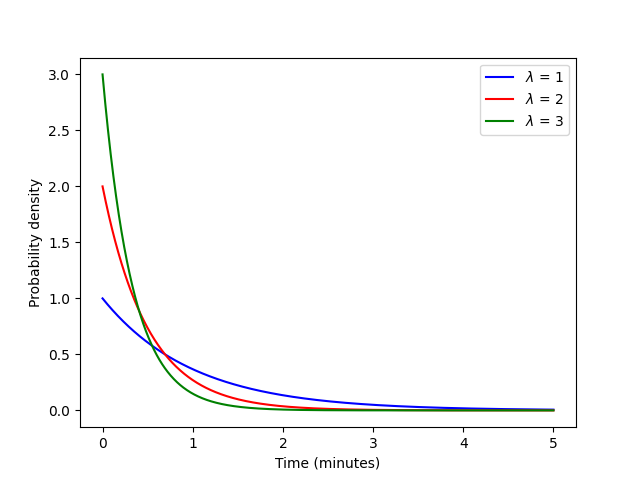
\includegraphics[width=0.5\textwidth]{pic/exponential_distribution.png}
    \caption{三个不同参数的指数分布图表。}
    \label{fig:exp_dist}
\end{figure}

% \begin{minted}[bgcolor=black!5!white,linenos=true]{python}
% ……
% \end{minted}

% \begin{listing}[ht]
%    \caption{指数分布图的PYTHON源码} % 设置图题
%    \inputminted[bgcolor=codebgcolor,linenos=true]{python}{pic/exponential_distribution.py} % 引用代码文件
% \end{listing}

\inputminted[bgcolor=codebgcolor,linenos=true]{python}{pic/exponential_distribution.py}

--------------------------------------------------------------------------------------------------
\subsubsection{中心极限定理}
设 $X_1, X_2, \dots, X_n$ 是独立同分布的随机变量,$E(X_i) = \mu$,$D(X_i) = \sigma^2 < \infty$,定义随机变量 $Z_n = \frac{\sum_{i=1}^{n}(X_i - \mu)}{\sigma \sqrt{n}}$,则有:
$$
\lim_{n\rightarrow\infty}P(Z_n\leq x) = \Phi(x),
$$
其中 $\Phi(x)$ 是标准正态分布的分布函数。
\\\\\\
举例:\\
中心极限定理是概率论的一个重要定理,它指出,对于任意分布的随机变量,其样本均值的分布会随着样本量的增大逐渐近似于正态分布。下面我用一个简单的例子来说明中心极限定理。

假设有一个硬币,正反面出现的概率分别为 0.5。现在我们抛掷这个硬币 200 次,每次记录正反面出现的情况,然后计算出这 200 次抛掷中正面朝上的次数,再将这个次数除以 200 得到一个概率值,表示正面朝上的概率。我们假设这个概率为 p。

我们重复上述过程很多次,每次得到一个概率值 p,然后记录下来。这样我们就得到了一堆概率值,可以计算它们的平均值和标准差。根据中心极限定理,当样本量足够大时,这些概率值的平均值应该近似于 p,而且这个平均值的分布应该趋近于正态分布。同时,这个平均值的标准差可以用来估计样本均值的精度。

举个具体的例子,假设我们重复上述过程 10,000 次,每次抛掷硬币 200 次,得到了 10,000 个概率值。我们计算这些概率值的平均值为 0.4999,标准差为 0.0356。这个平均值很接近于真实概率值 0.5,而且它的分布近似于正态分布。如果我们再增加样本量,比如抛掷硬币 1,000 次或者更多次,结果会更加接近正态分布。


--------------------------------------------------------------------------------------------------
\subsubsection{贝叶斯规则}
$ p(\mathbf{x} | \mathbf{y}) = \frac{p(\mathbf{y} | \mathbf{x})p(\mathbf{x})}{p(\mathbf{y})} $

--------------------------------------------------------------------------------------------------

\section{数值计算}
\subsection{上溢和下溢}

下溢:指数字的绝对值太小而无法用计算机中的浮点数表示。例如,当我们将一个非常接近于零的数乘以另一个非常接近于零的数时,结果可能会变得非常接近于零。在这种情况下,由于数字变得太小,计算机可能无法准确地表示它们,这导致结果存在误差。

上溢:指数字的绝对值太大而无法用计算机中的浮点数表示。例如,当我们将两个非常大的数相乘时,结果可能会变得非常大,超出了计算机可以表示的范围。这导致计算机无法将结果准确地存储,并返回一个特殊的错误代码或无穷大值。

--------------------------------------------------------------------------------------------------
\subsection{病态条件}
$ \kappa(\mathbf{X}) = \frac{\sigma_{max}}{\sigma_{min}} $  \\
其中,$ \kappa(\mathbf{X}) $ 表示矩阵 $\mathbf{X}$ 的病态条件,$\sigma_{max}​$和$\sigma_{min}​$ 表示 $\mathbf{X}$ 的最大和最小奇异值,分别对应矩阵的最大和最小特征值的平方根。

--------------------------------------------------------------------------------------------------
\subsection{基于梯度的优化方法}
偏导数:
$$\frac{\partial f}{\partial x_i}$$
梯度:
$$\vec{\nabla}f=\begin{pmatrix}\frac{\partial f}{\partial x_1} \\ \frac{\partial f}{\partial x_2} \\ ... \\ \frac{\partial f}{\partial x_n} \end{pmatrix}$$



--------------------------------------------------------------------------------------------------

二阶泰勒展开式  \\
$ f(x + \Delta x) = f(x) + f'(x)\Delta x + \frac{f''(x)}{2!}\Delta x^2 + \frac{f'''(x)}{3!}\Delta x^3 + ... $ \\

$ f(x+\Delta x) \approx f(x) + f'(x)\Delta x + \frac{1}{2}f''(x)(\Delta x)^2 $ \\

牛顿法:
$$f(x)\approx f(x_k)+\nabla f(x_k)^T(x-x_k)+\frac{1}{2}(x-x_k)^T\nabla^2f(x_k)(x-x_k)$$
--------------------------------------------------------------------------------------------------

简单的最小二乘习题:给定以下数据点 (1,1),(2,2),(3,3),(4,5),(5,5),试求通过这些数据点的最小二乘线性回归直线的方程,并计算该直线在 x=6 处的预测值。这个问题可以帮助学生更好地理解最小二乘法在线性回归中的应用。

解答:

我们可以通过下面的步骤来求解这个问题:

    首先,我们要计算数据点的均值向量 $\bar{x}$ 和 $\bar{y}$,它们分别表示 x 和 y 的平均值。在这个例子中,我们有:
$$
\begin{aligned}
    \bar{y} &= \frac{1+2+3+5+5}{5} = 3.2
\end{aligned}
$$
2. 接下来,我们可以计算 $x$ 和 $y$ 的样本协方差矩阵 $S_{xy}$ 和 $x$ 的样本方差 $S_x^2$。它们的计算公式分别为: 
$$\begin{aligned} 
    S_{xy} &= \frac{1}{n-1}\sum_{i=1}^n(x_i - \bar{x})(y_i - \bar{y}),\\ 
    S_x^2 &= \frac{1}{n-1}\sum_{i=1}^n(x_i - \bar{x})^2, 
\end{aligned}
$$ 
其中 $n$ 表示样本的数量。在这个例子中,我们有: 
$$
\begin{aligned} 
    S_{xy} &= \frac{(1-3)(1-3.2)+(2-3)(2-3.2)+(3-3)(3-3.2)+(4-3)(5-3.2)+(5-3)(5-3.2)}{5-1} = 2.3,\\ 
    S_x^2 &= \frac{(1-3)^2+(2-3)^2+(3-3)^2+(4-3)^2+(5-3)^2}{5-1} = 2.
\end{aligned}
$$ 
3. 然后,我们可以计算回归方程的斜率 $b$ 和截距 $a$,它们分别为: 
$$
\begin{aligned}
    b &= \frac{S_{xy}}{S_x^2} = 1.15,\\ 
    a &= \mathbf{\bar{y}} - b\mathbf{\bar{x}} = 0.55.
\end{aligned}
$$ 
因此,通过这些数据点的最小二乘线性回归直线的方程为 $y = 1.15x + 0.55$。 \\
4. 最后,我们可以使用回归方程来预测 $x=6$ 时的 $y$ 值,它可以通过将 $x$ 的值代入回归方程中得到: 
$$y = 1.15\times 6 + 0.55 = 7.45.$$ 
因此,在 $x=6$

--------------------------------------------------------------------------------------------------
\section{机器学习基础}
\setlength{\parindent}{20pt}
\setlength{\parindent}{0pt}
\setlength{\parindent}{20pt}
\indent

Tom Mitchell是一位著名的人工智能学家,他在他的一篇经典论文《机器学习》中给出了学习的定义:

"\textcolor{red}{\textbf{对于一类任务T和性能度量P,如果一个计算机程序在任务T上以性能度量P衡量的性能随着经验E的增加而自我完善,那么我们称这个计算机程序在从经验E中学习。}}"

\textit{任务T:包括一切机器可以执行的任务,如分类、回归、聚类等;}

\textit{性能度量P:指的是机器执行任务T的表现如何被衡量,例如在分类问题中正确率,回归问题中的均方误差;}

\textit{经验E:表示所学习的信息,可以是从实际经验中获得的数据集,也可以是人工构造出的数据集或先验知识。机器通过不断地从经验E中学习,自我完善,从而具有了更好的性能。}

这个定义概括了机器学习的基本概念和方法,是机器学习研究和应用的基础。


\subsection{估计量}
估计量是指根据样本数据来计算总体参数的量。在统计学中,由于我们往往无法对总体参数进行准确测量,需要使用估计量来对总体参数进行估计。常见的估计量包括样本均值、样本方差、样本比率等等。通过这些估计量,我们可以推断总体参数的值,并进行统计推断。
例子:假设我们想要估计某个城市的平均每天骑共享单车的人数。我们可以通过抽取一部分人群的每日骑行数据来进行估计。在这个例子中,我们可以计算出样本均值作为估计量,即每日骑行人数的平均值。

举个具体例子,我们抽取了50个人群的每日骑行数据,得到样本数据如下:

22, 32, 18, 25, 30, 28, 40, 20, 16, 24, 36, 33, 27, 29, 31, 19, 17, 21, 23, 26, 22, 16, 28, 24, 37, 30, 26, 19, 27, 35, 28, 18, 21, 23, 19, 25, 34, 27, 22, 18, 20, 29, 26, 23, 31, 20, 33, 25, 28, 19

通过对这些数据求平均值,我们可以得到样本均值为25.24。因此,我们可以使用25.24作为估计量来估计这个城市的平均每天骑共享单车的人数。另外,我们还可以计算出置信区间,比如95%置信区间来评估估计量的置信度,从而判断估计结果的可靠性。

--------------------------------------------------------------------------------------------------
\subsection{最大似然估计}


--------------------------------------------------------------------------------------------------
\end{document}